\section{Triển khai mạch điều khiển và mạch động lực cho hệ thống}
\subsection{Mạch điều khiển}
\begin{figure}[H]
    \centering
    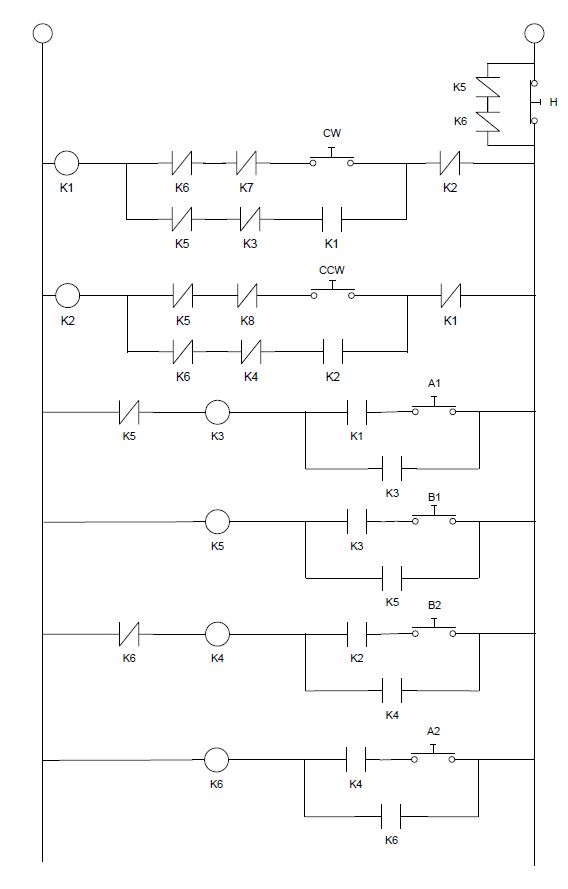
\includegraphics[width=0.8\textwidth]{pictures/control.png}
\end{figure}
\cleardoublepage
\subsection{Mạch động lực}
\begin{figure}[H]
    \centering
    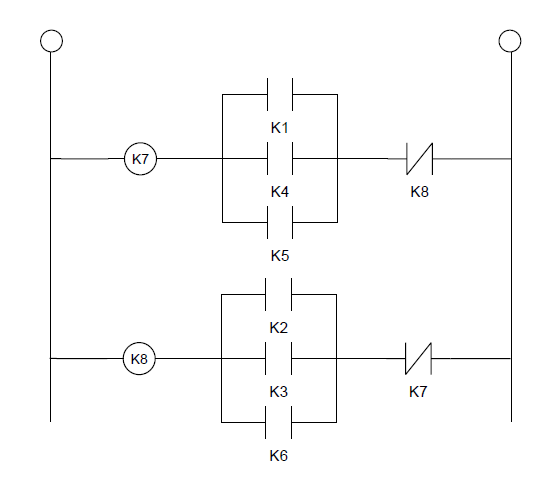
\includegraphics[width=0.6\textwidth]{pictures/power.png}
\end{figure}
\subsection{Bảng trạng thái của chiều quay động cơ}
\begin{center}
\begin{tabular}{|c|c|c|c|c|c|c|c|c|c|c|}
    \hline  
    Trạng thái & K1 & K2 & K3 & K4 & K5 & K6 & K7 & K8 & Chiều quay\\
    \hline
    1 & 1 & 0 & 0 & 0 & 0 & 0 & 1 & 0 & CW\\
    \hline
    2 & 0 & 1 & 0 & 0 & 0 & 0 & 0 & 1 & CCW\\
    \hline
    3 & 0 & 0 & 1 & 0 & 0 & 0 & 0 & 1 & CCW\\
    \hline
    4 & 0 & 0 & 0 & 1 & 0 & 0 & 1 & 0 & CW\\
    \hline
    5 & 0 & 0 & 0 & 0 & 1 & 0 & 1 & 0 & CCW\\
    \hline
    6 & 0 & 0 & 0 & 0 & 0 & 1 & 0 & 1 & CW\\
    \hline
\end{tabular}
\end{center}
\subsection{Nguyên lý hoạt động}
\hspace*{0.5cm}Khi nhấn nút CW bàn sẽ xoay theo chiều kim đồng hồ (H -> A theo chiều kim đồng hồ, A -> B ngược chiều kim đồng hồ, B -> H theo chiều kim đồng hồ)\\

Còn khi nhấn nút CCW bàn sẽ xoay theo ngược chiều kim đồng hồ (H -> B theo chiều kim đồng hồ, B -> A ngược chiều kim đồng hồ, A -> H theo chiều kim đồng hồ)\\

Vì 2 trường hợp tương ứng với 2 nút nhấn có nguyên lý hoạt động tương tự nhau nên ở đây ta xét ví dụ khi nhấn nút CW:
\begin{itemize}
    \item Khi nút CW được nhấn, cuộn coil K1 được kích, 2 tiếp điểm thường mở của K1 đóng lại, đồng thời tiếp điểm thường đóng của K1 mở ra ở nhánh có nút CCW để khóa trái 2 nút.
\end{itemize}
\begin{figure}[H]
    \centering
    \rotatebox{270}{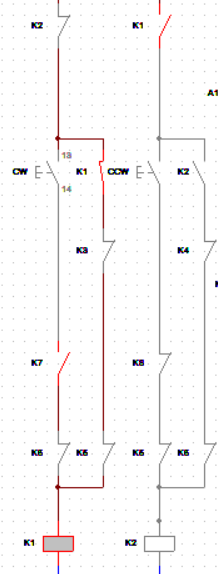
\includegraphics[width=0.3\textwidth]{pictures/nhannut.png}}
\end{figure}
\begin{itemize}
    \item Đồng thời cặp tiếp điểm thường đóng K1 ở mạch động lực đóng lại làm cuộn coil K7 được kích, động cơ quay theo chiều kim đồng hồ.
\end{itemize}
\begin{figure}[H]
    \centering
    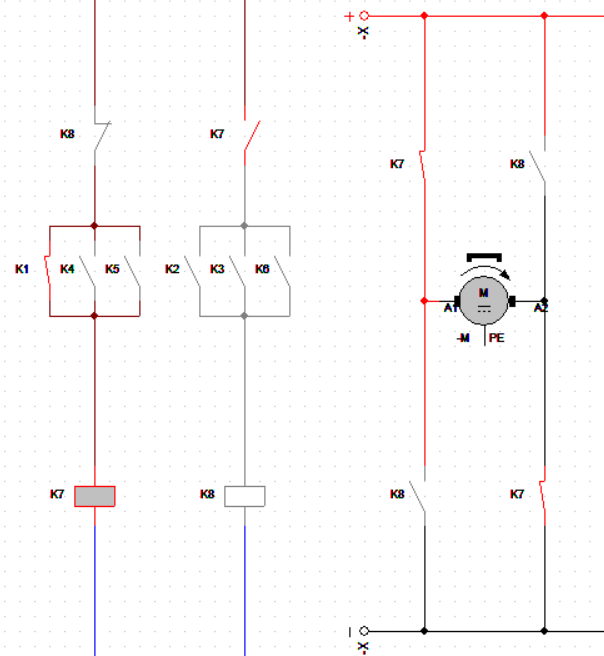
\includegraphics[width=0.5\textwidth]{pictures/kichK1.png}
\end{figure}
\begin{itemize}
    \item Cặp tiếp điểm K1 ở nhánh có cảm biến tại vị trí A đóng lại để khi có tín hiệu từ cảm biến, cuộn coil K3 sẽ được kích.
\end{itemize}
\begin{figure}[H]
    \centering
    \rotatebox{270}{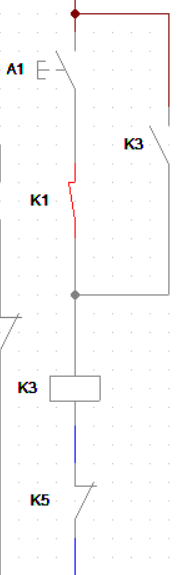
\includegraphics[width=0.3\textwidth]{pictures/denA.png}}
\end{figure}
\begin{itemize}
    \item Khi có tín hiệu từ cảm biến ở vị trí A, cuộn coil K3 được kích, cặp tiếp điểm thường đóng ở nhánh có nút CW mở ra để cuộn coil K1 ngưng kích từ đó cuộn coil K7 cũng ngưng kích theo.
    \item Cặp tiếp điểm thường mở K3 ở mạch động lực đóng lại, cuộn coil K8 được kích động cơ quay ngược chiều kim đồng hồ. 
\end{itemize}
\begin{figure}[H]
    \centering
    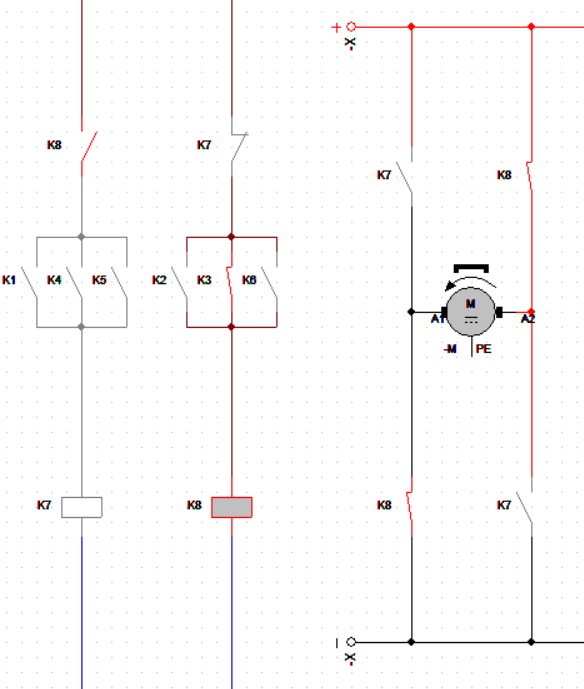
\includegraphics[width=0.5\textwidth]{pictures/kichK3.png}
\end{figure}
\begin{itemize}
    \item Cặp tiếp điểm thường mở của K3 ở nhánh có cảm biến tại vị trí B đóng lại để khi có tín hiệu từ cảm biến, cuộn coil K5 sẽ được kích.
\end{itemize}
\begin{figure}[H]
    \centering
    \rotatebox{270}{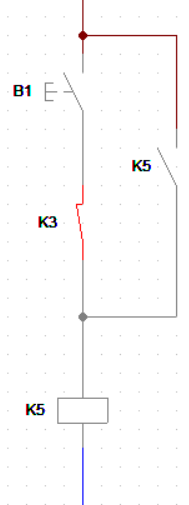
\includegraphics[width=0.3\textwidth]{pictures/denB.png}}
\end{figure}
\begin{itemize}
    \item Khi có tín hiệu từ cảm biến ở vị trí B, cuộn coil K5 được kích, cặp tiếp điểm thường đóng ở nhánh có nút CW mở ra để cuộn coil K3 ngưng kích từ đó cuộn coil K8 cũng ngưng kích theo.
    \item Cặp tiếp điểm thường đóng K5 ở mạch động lực đóng lại, cuộn coil K7 được kích động cơ quay theo chiều kim đồng hồ.
\end{itemize}
\begin{figure}[H]
    \centering
    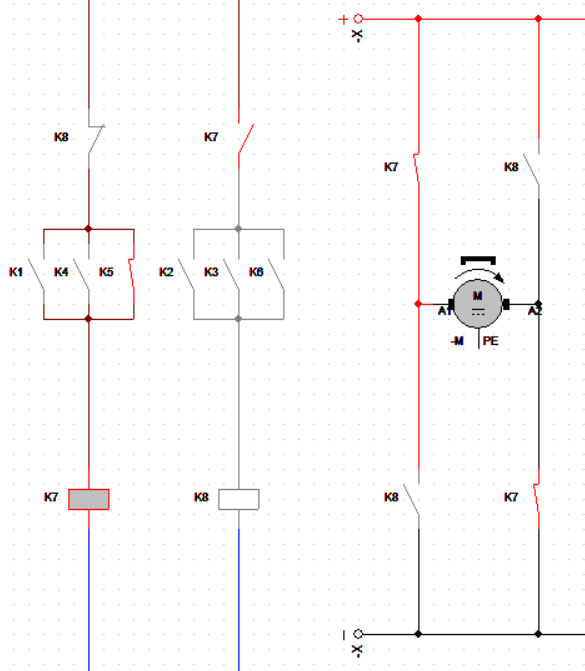
\includegraphics[width=0.5\textwidth]{pictures/kichK5.png}
\end{figure}
\begin{itemize}
    \item Một cặp tiếp điểm thường đóng của K5 ở nhánh có cảm biến tại vị trí H mở ra để khi có tín hiệu từ cảm biến, toàn bộ mạch điện sẽ được ngắt điện và trở về trạng thái ban đầu, kết thúc 1 chu kỳ.
\end{itemize}
\begin{figure}[H]
    \centering
    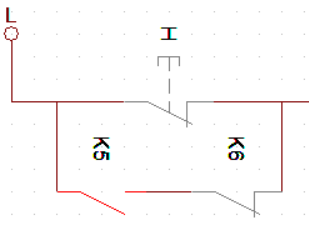
\includegraphics[width=0.5\textwidth]{pictures/denH.png}
\end{figure}
\begin{itemize}
    \item Khi 1 trong 2 nút được nhấn, hệ thống tiếp tục hoạt động theo nguyên lý trên.
\end{itemize}
\cleardoublepage